% This file was converted to LaTeX by Writer2LaTeX ver. 1.0.2
% see http://writer2latex.sourceforge.net for more info
\documentclass[twoside,letterpaper]{article}
\usepackage{amsmath}
\usepackage{amssymb,amsfonts,textcomp}
\usepackage{array}
\usepackage[english]{babel}
\usepackage[small,bf]{caption}
\usepackage{color}
\usepackage[T1]{fontenc}
\usepackage{hhline}
\usepackage{hyperref}
\usepackage[latin1]{inputenc}
\usepackage{multirow}
\usepackage{supertabular}
\hypersetup{pdftex, colorlinks=true, linkcolor=blue, citecolor=blue, filecolor=blue, urlcolor=blue, pdftitle=SYSTEMS AND SOFTWARE REQUIREMENTS SPECIFICATION (SSRS) TEMPLATE, pdfauthor=Clinton Jeffery, pdfsubject=, pdfkeywords=}
\usepackage[pdftex]{graphicx}
% Outline numbering
\setcounter{secnumdepth}{5}
\renewcommand\thesection{\arabic{section}}
\renewcommand\thesubsection{\arabic{section}.\arabic{subsection}}
\renewcommand\thesubsubsection{\arabic{section}.\arabic{subsection}.\arabic{subsubsection}}
\renewcommand\theparagraph{\arabic{section}.\arabic{subsection}.\arabic{subsubsection}.\arabic{paragraph}}
\renewcommand\thesubparagraph{\arabic{section}.\arabic{subsection}.\arabic{subsubsection}.\arabic{paragraph}.\arabic{subparagraph}}
\makeatletter
\newcommand\arraybslash{\let\\\@arraycr}
\makeatother
% Page layout (geometry)
\setlength\voffset{-1in}
\setlength\hoffset{-1in}
\setlength\topmargin{0.5in}
\setlength\oddsidemargin{1in}
\setlength\evensidemargin{1in}
\setlength\textheight{8.278in}
\setlength\textwidth{6.5in}
\setlength\footskip{0.561in}
\setlength\headheight{0.5in}
\setlength\headsep{0.461in}
% Footnote rule
\setlength{\skip\footins}{0.0469in}
\renewcommand\footnoterule{\vspace*{-0.0071in}\setlength\leftskip{0pt}\setlength\rightskip{0pt plus 1fil}\noindent\textcolor{black}{\rule{0.25\columnwidth}{0.0071in}}\vspace*{0.0398in}}
% Pages styles
\makeatletter
\newcommand\ps@Standard{
  \renewcommand\@oddhead{\rmfamily University of Idaho CS Department Instructional Use\hfill \hfill NOT FOR RELEASE}
  \renewcommand\@evenhead{\@oddhead}
  \renewcommand\@oddfoot{\foreignlanguage{english}{\textcolor{black}{SSRS Page }}\foreignlanguage{english}{\textcolor{black}{\thepage{}}}}
  \renewcommand\@evenfoot{\@oddfoot}
  \renewcommand\thepage{\arabic{page}}
}

%% ENVIRONMENT TO SINGLE-SPACE ENUMERATION LINES
\newenvironment{my_enumerate}{
\begin{enumerate}
  \setlength{\itemsep}{1pt}
  \setlength{\parskip}{0pt}
  \setlength{\parsep}{0pt}}{\end{enumerate}
}
%% ENVIRONMENT TO SINGLE-SPACE ITEMIZED LINES
\newenvironment{my_itemize}{
\begin{itemize}
  \setlength{\itemsep}{1pt}
  \setlength{\parskip}{0pt}
  \setlength{\parsep}{0pt}}{\end{itemize}
}

\newcommand\ps@Convertviii{
  \renewcommand\@oddhead{}
  \renewcommand\@evenhead{\@oddhead}
  \renewcommand\@oddfoot{}
  \renewcommand\@evenfoot{\@oddfoot}
  \renewcommand\thepage{\arabic{page}}
}
\newcommand\ps@Convertvii{
  \renewcommand\@oddhead{}
  \renewcommand\@evenhead{\@oddhead}
  \renewcommand\@oddfoot{}
  \renewcommand\@evenfoot{\@oddfoot}
  \renewcommand\thepage{\arabic{page}}
}
\newcommand\ps@Convertvi{
  \renewcommand\@oddhead{}
  \renewcommand\@evenhead{\@oddhead}
  \renewcommand\@oddfoot{}
  \renewcommand\@evenfoot{\@oddfoot}
  \renewcommand\thepage{\arabic{page}}
}
\newcommand\ps@Convertv{
  \renewcommand\@oddhead{}
  \renewcommand\@evenhead{\@oddhead}
  \renewcommand\@oddfoot{}
  \renewcommand\@evenfoot{\@oddfoot}
  \renewcommand\thepage{\arabic{page}}
}
\newcommand\ps@Convertiv{
  \renewcommand\@oddhead{}
  \renewcommand\@evenhead{\@oddhead}
  \renewcommand\@oddfoot{}
  \renewcommand\@evenfoot{\@oddfoot}
  \renewcommand\thepage{\arabic{page}}
}
\newcommand\ps@Convertii{
  \renewcommand\@oddhead{}
  \renewcommand\@evenhead{\@oddhead}
  \renewcommand\@oddfoot{}
  \renewcommand\@evenfoot{\@oddfoot}
  \renewcommand\thepage{\arabic{page}}
}
\newcommand\ps@FirstPage{
  \renewcommand\@oddhead{}
  \renewcommand\@evenhead{\@oddhead}
  \renewcommand\@oddfoot{}
  \renewcommand\@evenfoot{\@oddfoot}
  \renewcommand\thepage{\arabic{page}}
}
\makeatother
\pagestyle{Standard}
\setlength\tabcolsep{1mm}
\renewcommand\arraystretch{1.3}
% footnotes configuration
\makeatletter
\renewcommand\thefootnote{\arabic{footnote}}
\makeatother
\title{SYSTEMS AND SOFTWARE REQUIREMENTS SPECIFICATION (SSRS) TEMPLATE}
\author{Clinton Jeffery}
\date{2010-11-18T11:33:37.30}
\begin{document}




\clearpage
{\centering\bfseries
SYSTEMS AND SOFTWARE \ REQUIREMENTS SPECIFICATION (SSRS) FOR
\par}


\bigskip

{\centering\bfseries
Phunctional UML Editor
\\(pUML)
\par}


\bigskip


\bigskip


\bigskip

\begin{figure}
\centering

\includegraphics[width=3.5in]{uidahologo.jpg}
\end{figure}

\bigskip


\bigskip

{\centering\bfseries
Version 7.0
\par}

{\centering\bfseries
April 9, 2012
\par}


\bigskip


\bigskip

{\centering\bfseries
Prepared for:
\par}
{\centering\bfseries
Dr. Clint Jeffery
\par}

\bigskip


\bigskip

{\centering\bfseries
Prepared by:
\par}

{\centering\bfseries
Josh Armstrong
\\Zach Curtis
\\Brian Bowles
\\Logan Evans
\\Jeremy Klas
\\Nathan Krussel
\\Maxine Major
\\Morgan Weir
\\David Wells
\par}

{\centering\bfseries
University of Idaho
\par}

{\centering\bfseries
Moscow, ID \ 83844-1010
\par}

\clearpage{\centering\bfseries
pUML SSRS
\par}


\bigskip





{\centering\bfseries RECORD OF CHANGES \par}


\bigskip

\begin{flushleft}
\tablehead{}
\begin{supertabular}[c]{|m{0.75in}|m{1.0in}|m{1.5in}|m{0.25in}|m{2in}|c|}
\hline

\centering \bfseries Change
\centering \bfseries Number
&

\centering \bfseries Date
\par
&

\centering \bfseries Location of change\newline
\centering \bfseries(e.g., page or figure \#)
&

\centering \bfseries A\newline
\centering \bfseries M\newline
\centering \bfseries D  
&

\centering \bfseries Brief description\newline
\centering \bfseries of change
&
\bfseries Initials
\\\hline

\centering 1
& 12/10/2011
& ~
& \centering A
& Text material for section 3 of the SSRS document.
& LE

\\\hline
\centering 2
& 01/17/2012
& ~
& \centering A
& Added updated SSRS/SSDD pdf and TeX files
& MM

\\\hline
\centering 3
& 02/01/2012
& ~
& \centering M
& Updated SSRS and SSDD
& MM

\\\hline
\centering 4
& 02/15/2012
& ~
& \centering M
& Use cases expanded and descriptions added
& MM

\\\hline
\centering 5
& 02/23/2012
& ~
& \centering M
& Use case descriptions completed
& MM

\\\hline
\centering 6
& 04/04/2012
& ~
& \centering M
& Revised use case descriptions
& MW

\\\hline
\centering 7
& 04/09/2012
& ~
& \centering A
& Requirements update
& MM
\\\hline
\end{supertabular}
\end{flushleft}










{
\foreignlanguage{english}{*}\foreignlanguage{english}{\textbf{A}}\foreignlanguage{english}{
- ADDED
\ }\foreignlanguage{english}{\textbf{M}}\foreignlanguage{english}{ -
MODIFIED
\ }\foreignlanguage{english}{\textbf{D}}\foreignlanguage{english}{ -
DELETED}}

\clearpage{\centering\bfseries
\foreignlanguage{english}{\MakeUppercase{\ }}\foreignlanguage{english}{\MakeUppercase{pUML SSRS}}
\par}

{\centering\bfseries
TABLE OF CONTENTS
\par}


\bigskip

{\bfseries
Section\ \ Page}

\setcounter{tocdepth}{9}
\renewcommand\contentsname{}
\tableofcontents

\bigskip








\clearpage\clearpage\setcounter{page}{1}\pagestyle{Convertii}
\section[Introduction]{\rmfamily\bfseries
Introduction}

\subsection[IDENTIFICATION]{\rmfamily\bfseries
IDENTIFICATION}
{
The software system being considered for development is referred to as Phunctional UML Editor (pUML). \ The customer providing specifications
for the system is Dr. Clint Jeffery at the University of Idaho. \ The ultimate
customer, or end-user, of the system will be University of Idaho Computer Science students and/or faculty. \ This is a new project effort, so the version under development is version 0.0.}

\subsection[PURPOSE]{\rmfamily\bfseries
PURPOSE}
{
The purpose of the system under development is to create and store UML diagrams.
\ While the system will be used by Computer Science students at the University of Idaho,
this document is intended to be read and understood by UICS software
designers and coders.}

\subsection[SCOPE]{\rmfamily\bfseries
SCOPE}
{
The pUML software was conceptualized as a Software Engineering class project, and was launched in September 2011 .  The pUML project is as of the date of this SSRS publication, incomplete, and has yet no aquirers, users, support agencies at this time. Upon completion, the pUML software will be available only for distribution to the University of Idaho Computer Science department, and will be supported by the development team. }

\subsection[DEFINITIONS, ACRONYMS, AND
ABBREVIATIONS]{\rmfamily\bfseries
DEFINITIONS, ACRONYMS, AND ABBREVIATIONS}

\bigskip

\begin{flushleft}
\tablehead{}
\begin{supertabular}{|m{1.3587599in}|m{5.00806in}|}
\hline
\centering \bfseries Term or
Acronym &
\centering\arraybslash \bfseries
Definition\\\hline
 Alpha test &
 Limited release(s) to selected,
outside testers\\\hline
 Beta test &
 Limited release(s) to cooperating
customers wanting early access to developing systems\\\hline
 Final test &
 aka, Acceptance test, release of
full functionality to customer for approval
\\\hline
 SSDD &
 System and Software Design Document\\\hline
 SSRS &
 System and Software Requirements
Specification\\\hline
~
 &
~
\\\hline

\end{supertabular}
\end{flushleft}
\subsection[REFERENCES]{\rmfamily\bfseries
REFERENCES}
{
The pUML requirements have been met in the following two documents: 

\begin{enumerate}
\item Test Plan (TP)
\item System and Software Design Description (SSDD)
\end{enumerate}

}

\subsection[OVERVIEW AND RESTRICTIONS]{\rmfamily\bfseries
OVERVIEW AND RESTRICTIONS}
{
This document is for limited release only to UI CS personnel working on
the project.}


\bigskip

{
Section 2 of this document describes the system under development from a
holistic point of view. \ Functions, characteristics, constraints,
assumptions, dependencies, and overall requirements are defined from
the system-level perspective.}


\bigskip

{
Section 3 of this document describes the specific requirements of the
system being developed. \ Interfaces, features, and specific
requirements are enumerated and described to a degree sufficient for a
knowledgeable designer or coder to begin crafting an architectural
solution to the proposed system.}


\bigskip

{
Section 4 provides the requirements traceability information for the
project. \ Each feature of the system is indexed by the SSRS
requirement number and linked to its SDD and test references.}


\bigskip

{
Sections 5 and up are appendices including original information and
communications used to create this document.}











\clearpage\section[OVERALL DESCRIPTION]{\rmfamily\bfseries
OVERALL DESCRIPTION}

\subsection[PRODUCT PERSPECTIVE]{\rmfamily\bfseries
PRODUCT PERSPECTIVE}
{
This product is independent of any other product, and as such, is self-contained.
}

\subsubsection[PRODUCT FUNCTIONS]{\rmfamily\bfseries
PRODUCT FUNCTIONS}

This product's primary function is to allow the user to create UML diagrams, edit existing diagrams, and store and retrieve them.
\newline Features to be tested include all objects, connectors, and associated functionality, Open/Save/Restore functionality, and all diagram types load properly. The specific requirements for the UML diagram editor are itemized below.


\subsubsection[MENU/OPTIONS MENU/MAINWINDOW]{\bfseries MENU/OPTIONS MENU/MAINWINDOW} 

\begin{itemize}
\item Options window appears at pUML startup.
\item When the options window is closed with no selections made, the pUML main window remains.
\item When "New" is selected, options window appears.
\item When "Open" is selected, an explorer window appears.
\item When "Save" is selected: refer to subsection 2.1.6.
\item When "Save As.." is selected: refer to subsection 2.1.6.
\item When Exit is clicked:
\begin{itemize}
\item If all currently open diagrams are saved, pUML exits.
\item If any open diagram is not saved, refer to subsection 2.1.6.
\end{itemize}

\end{itemize}



\subsubsection[OBJECTS]{\bfseries OBJECTS} 

All objects should perform or have the following tasks performed on them in a consistent manner in the following cases: 
\begin{itemize}
	\item Objects can be created.
	\item Objects can be deleted.
\begin{itemize}
\item Any associated connectors must also be deleted.
\item All associated text and descriptions must also be deleted.
\end{itemize}
	\item Objects can be selected.
	\item Objects can be de-selected.
	\item Objects can be moved after they have been placed
\begin{itemize}
\item Objects moved retain the new location after the associated diagram is saved, closed, and restored.
\item All text and descriptions associated with the object move with the object to the same location in relation to the object.
\end{itemize}
\item Objects can accept an indefinite number of connection lines.
	\item The object's properties may be modified.
\begin{itemize}
\item Description or contents may be modified an indefinite number of times.
\end{itemize}
	\item The object will automatically resize to fit the contents.
\end{itemize}

\bigskip

\subsubsection[CONNECTORS]{\bfseries CONNECTORS}

All connectors should perform or have the following tasks performed on them in a consistent manner in the following cases: 
\begin{itemize}
\item Connectors can be created.
\begin{itemize}
\item Only one connector may exist between any two objects.
\item Only one self connector may exist per object.
\end{itemize}
\item Connectors can be deleted.
\item Connectors can be selected.
\item Connectors can be de-selected.
\item Connectors cannnot be moved from one object and placed onto another. 
\item If an object a connector is attached to moves, the connector's endpoint attached to that object will move with that object. 
\begin{itemize}
\item Connectors moved retain the new configuration with the same integrity as the previous configuration.
\item All text and descriptions associated with the connector move with the connector to the same location in relation to the connector as before.
\end{itemize}
\item The connector's properties may be modified.
\begin{itemize}
\item Line description may be modified an indefinite number of times.
\end{itemize}
\end{itemize}

\bigskip

\subsubsection[OPEN]{\bfseries OPEN}

Once the pUML software has been launched, files may be opened if the following criteria are met:

\begin{itemize}
\item The file type is of pUML type.
\item The file name is legitimate.
\item The file is not already open in pUML.
\end{itemize}

\newline Note: The cases listed above are ensured by QT, and will not be tested.
\newline 

\begin{itemize}
\item When a file is opened, the diagram loads into a new tab.
\item The toolbar is updated with that diagram's objects and connectors.
\item All objects and connectors in the file are in the exact same state and configuration as when the file had been previously saved.
\item The file may be modified (edited).
\begin{itemize}
\item Objects may be added or removed.
\item Connectors may be added or removed.
\end{itemize}
\item The file may be saved.
\item The file may be closed.
\end{itemize}

\bigskip

\subsubsection[SAVE]{\bfseries SAVE/SAVE AS}

The Save and Save As functions may be invoked if the following criteria are met: 
\begin{itemize}
\item A diagram is open in pUML.
\end{itemize}

\newline Save/Save As functionality:
\newline
\begin{itemize}
\item A diagram may be saved regardless of whether it is new or previously saved.
\item A diagram may be saved whether or not it has been modified. (e.g., a blank diagram may be saved)
\item If a diagram has been previously saved, pUML will automatically write over the saved file's contents. The modified diagram will be saved at the original location of the diagram under the original name.
\item If a diagram has not been previously saved, Save As will automatically occur.
\begin{itemize}
\item The Save-As dialog will load.
\item The user must select an appropriate file name and storage location. 
\item The diagram will be stored at the location and under the name the user has entered.
\end{itemize}
\end{itemize}


\bigskip


\subsubsection[RESTORE]{\bfseries RESTORE}

If the user opens a pUML diagram file, restore functionality will occur as follows:
\begin{itemize}
\item If the pUML software is not already loaded, it will load.
\item A new tab will open, and the previously saved diagram will appear in the tab.
\item This newly-loaded diagram will retain all the stored information from the previous save.
\end{itemize}


\bigskip

\subsubsection[DIAGRAM TYPES]{\bfseries DIAGRAM TYPES}

\begin{itemize}
\item pUML diagrams may be of only one diagram type. (There are no legitimate UML diagrams that combine elements of more than one diagram type)
\item Diagram-specific objects and connectors will be the only ones displayed in the toolbar for a specific diagram type.
\item The type of the diagram will be saved with a diagram file, so that a diagram may not be loaded into a tab with a different diagram type.
\end{itemize}


\bigskip

\subsubsection[TAB FUNCTIONALITY]{\bfseries TAB FUNCTIONALITY}

\begin{itemize}
\item Except for the initial loading of pUML (initial options window view), at least one tab must be open at any time.
\item If all tabs are closed, pUML exits.
\item If the diagram loaded into a tab is saved, clicking the ``X'' will close the tab.
\item If the diagram loaded into a tab is not saved, and the ``X'' is clicked: refer to subsection 2.1.6.
\item pUML will permit an indefinite number of tabs to be opened at any time, but this may consume a disproportionate amount of resources.
\end{itemize}



\bigskip




}

\subsection[USER CHARACTERISTICS]{\rmfamily\bfseries
USER CHARACTERISTICS}
{
The intended user for the pUML software are software engineers and computer science students with a prior knowledge of UML. This user is already familiar with computers and generally has some experience in programming languages.
}

\subsection[CONSTRAINTS]{\rmfamily\bfseries
CONSTRAINTS}
{
Since the pUML project was developed as a class assignment,
further development of this project will halt if the University of Idaho faculty overseeing this project decide that this project should to no longer continue.
}

\subsection[ASSUMPTIONS AND DEPENDENCIES]{\rmfamily\bfseries
ASSUMPTIONS AND DEPENDENCIES}
{
The requirements for the pUML software were decided upon by University of Idaho Computer Science Department faculty.  Any further direction this project may take will depend on their decisions. As of this revision, it is currently undecided if this project will be maintained after the corresponding course has concluded. 
}




\subsection[SYSTEM LEVEL (NON{}-FUNCTIONAL)
REQUIREMENTS]{\rmfamily\bfseries
SYSTEM LEVEL (NON-FUNCTIONAL) REQUIREMENTS}

\subsubsection[Site dependencies]{\rmfamily\bfseries
Site dependencies}
{
The pUML software has no dependencies on any external resources, such as internet access, etc..
Any modern operating system (2008+) should be sufficient to support the pUML software,
and since this software is cross-platform, there should be no complications.
}

\subsubsection[Safety, security and privacy requirements]{\rmfamily\bfseries
Safety, security and privacy requirements}
{
There are no safety, security or privacy requirements at this time.
}

\subsubsection[Performance requirements]{\rmfamily\bfseries
Performance requirements}
{
This software is to be supported on one terminal per install, and since there are no current
 limitations applying to product distribution, it may be installed on a theoretically infinite 
number of terminals. This software is not designed to be remotely accessed, and as a result, 
one user per session is recommended as well.  The software has not been tested to determine 
efficient transaction times as of the date of this SSRS publication.
}

\subsubsection[System and software quality]{\rmfamily\bfseries System
and software quality}
{
The fully developed software should be available for use and reliably handle all requests 98 
percent of the time.  The software can currently handle saving, diagram selection, allow for 
editing of multiple diagrams at a time, diagram component deletion, diagram component labeling, 
and loading of saved diagrams.
}

\subsubsection[Packaging and delivery requirements]{\rmfamily\bfseries
Packaging and delivery requirements}
{
The executable system and all associated documentation (i.e., SSRS, SSDD, code listing, test plan (data and results), and user manual) will be delivered to the customer on CD{\textquoteright}s and/or via email, as
specified by the customer at time of delivery. \ Although the user will be kept informed of progress via the Mercurial repository throughout the
system development process, the final, edited version of the above
documents will accompany the final, accepted version of the executable
system.}

\subsubsection[Personnel{}-related requirements]{\rmfamily\bfseries
Personnel-related requirements}
{
The system under development has no special personnel-related
characteristics. }

\subsubsection[Training{}-related requirements]{\rmfamily\bfseries
Training-related requirements}
{
A user manual will be included in this project to aid users who have difficulty intuiting the proper action to produce the corresponding outcome.
}

\subsubsection[Logistics{}-related requirements]{\rmfamily\bfseries
Logistics-related requirements}
{
The pUML software is intended for use on University of Idaho Computer Science department computers as well as computer science students' personal computers including, at a minimum, operating systems Windows 7, Mac OSX, and Linux.
Any minimum hardware requirements lie outside the scope of the resources available,
and there will be no software application dependencies at the time of release.
}

\subsubsection[Precedence and criticality of requirements]{\rmfamily\bfseries
Precedence and criticality of requirements}
{
System and software quality are the primary focus of our software development. All additional features and functionality are secondary. 
}












\clearpage\section[SPECIFIC REQUIREMENTS]{\rmfamily\bfseries
SPECIFIC REQUIREMENTS}

\subsection[EXTERNAL INTERFACE REQUIREMENTS]{\rmfamily\bfseries
EXTERNAL INTERFACE REQUIREMENTS}

\subsubsection[Hardware Interfaces]{\rmfamily\bfseries
Hardware Interfaces}
{
\foreignlanguage{english}{\ }\foreignlanguage{english}
{
Any computing system capable of running Linux or Windows 7.}}

\subsubsection[Software Interfaces]{\rmfamily\bfseries
Software Interfaces}
{ \foreignlanguage{english}{\ }\foreignlanguage{english}
{
Either a Linux or Windows 7 operating system to guarantee functionality.
}}

\subsubsection[User Interfaces]{\rmfamily\bfseries
User Interfaces}
{
\foreignlanguage{english}{\ }\foreignlanguage{english}
{
- Monitor
\\- Keyboard
\\- Mouse}}

\subsubsection[Other Communication
Interfaces]{\rmfamily\bfseries
Other Communication Interfaces}
{
\foreignlanguage{english}{\ }\foreignlanguage{english}{No other interfaces are required. }}





\clearpage\setcounter{page}{1}\pagestyle{Convertv}

\subsection[SYSTEM FEATURES]{\rmfamily\bfseries
SYSTEM FEATURES}


\subsubsection{Use Cases and Descriptions}
{The following use cases represent three different stages at which options will be available to the user.}

\bigskip
\bigskip

% ************************************
% LAUNCH USE CASE & DESCRIPTIONS
% ************************************
\paragraph[\ Use Category]
{\ Launch} {These options will be available to the user upon the immediate launch of pUML.}



%%% EXIT PROGRAM USE CASE DESCRIPTION
\begin{flushleft}
\tablehead{}
\begin{tabular}{|m{2.0in} m{5.0in}|}
\hline
{\bfseries\emph{Use Case Name}}
& {\bfseries Exit Program}
\\\hline
\emph{Participating Actor}
& User
\\\hline
\emph{Flow of Events}
& \begin{my_enumerate}
\item User clicks X.
\item If a file is open, program checks to see if it is saved.  If no files are open, simply exits.
\item Program Exits.
\end{my_enumerate}
\\\hline
\emph{Entry Condition}
&
User initiates File menu option ``Close Program'' or clicks X in the corner of the window.
\\\hline
\emph{Exit Condition}
& File is successfully saved and the program exits.
\\\hline
\emph{Quality Requirements}
& File must be saved prior to exiting, or changes must be discarded prior to exiting.
\\\hline
\end{tabular}
\end{flushleft}
\bigskip

\clearpage

% ************************************
% NEW PROJECT USE CASE & DESCRIPTIONS
% ************************************
\paragraph[\ Use Category]
{\ New Project} 
{The user has selected to start a new UML project.}


%%% CREATE NEW DIAGRAM USE CASE DESCRIPTION
\begin{flushleft}
\tablehead{}
\begin{tabular}{|m{2.0in} m{5.0in}|}
\hline
{\bfseries\emph{Use Case Name}}
& {\bfseries Create New Diagram }
\\\hline
\emph{Participating Actor}
& User
\\\hline
\emph{Flow of Events}
& \begin{my_enumerate}
\item The user selects new file from menu.
\item Program requests user select a diagram type
(includes ChooseDiagramType use case).
\item The program responds by creating a new file with a blank drawing canvas.
\end{my_enumerate}
\\\hline
\emph{Entry Condition}
& User selects New File from commands
\\\hline
\emph{Exit Condition}
& Program successfully opens new file
\\\hline
\emph{Quality Requirements}
& TBD
\\\hline
\end{tabular}
\end{flushleft}
\bigskip

%%% CHOOSE DIAGRAM TYPE USE CASE DESCRIPTION
\begin{flushleft}
\tablehead{}
\begin{tabular}{|m{2.0in} m{5.0in}|}
\hline
{\bfseries\emph{Use Case Name}}
& {\bfseries Choose Diagram Type}
\\\hline
\emph{Participating Actor}
& User 
\\\hline
\emph{Flow of Events}
& \begin{my_enumerate}
\item User selects a diagram type.
\item Program loads and displays only objects for the selected diagram type.
\end{my_enumerate}
\\\hline
\emph{Entry Condition}
& Included from New Diagram use case
\\\hline
\emph{Exit Condition}
& Included from New Diagram use case
\\\hline
\emph{Quality Requirements}
& Toolbar loads only diagram specific objects and connectors.
\\\hline
\end{tabular}
\end{flushleft}
\bigskip

\clearpage


% ************************************
% OPEN PROJECT USE CASE & DESCRIPTIONS
% ************************************
\paragraph[\ Use Category]
{\ Open Project} {These options will be available to the user after choosing to open an existing UML project.}

%%% OPEN EXISTING DIAGRAM USE CASE DESCRIPTION
\begin{flushleft}
\tablehead{}
\begin{tabular}{|m{2.0in} m{5.0in}|}
\hline
{\bfseries\emph{Use Case Name}}
& {\bfseries Open Existing Diagram}
\\\hline
\emph{Participating Actor}
& User
\\\hline
\emph{Flow of Events}
& \begin{my_enumerate}
\item User selects Open File from menu.
\item Program opens an explorer window.
\item User selects a file.
\item Program loads selected file into program
\end{my_enumerate}
\\\hline
\emph{Entry Condition}
& User selects Open File from menu.
\\\hline
\emph{Exit Condition}
& File is successfully opened.
\\\hline
\emph{Quality Requirements}
& User selected file must be able to be opened in pUML.
\\\hline
\end{tabular}
\end{flushleft}
\bigskip

\clearpage

% ************************************
% NEW DIAGRAM USE CASE & DESCRIPTIONS
% ************************************
\paragraph[\ Use Category]
{\ New Diagram} {These options will be available to the user upon choosing to create a new UML diagram.}

%%% SAVE DIAGRAM USE CASE DESCRIPTION
\begin{flushleft}
\tablehead{}
\begin{tabular}{|m{2.0in} m{5.0in}|}
\hline
{\bfseries\emph{Use Case Name}}
& {\bfseries Save File}
\\\hline
\emph{Participating Actor}
& User
\\\hline
\emph{Flow of Events}
& \begin{my_enumerate}
  \item The user opens the File menu and selects ``Save.''
  \item Program saves file under current file name 
\begin{my_enumerate}
\item If file has not been previously saved, program initiates Save As use case. 
\item If file has been previously saved, the program saves the file at its existing location under its existing name.
\end{my_enumerate}
\end{my_enumerate}
\\\hline
\emph{Entry Condition}
& User selects ``Save File'' from main menu or clicks Save button.
\\\hline
\emph{Exit Condition}
& File is successfully saved
\\\hline
\emph{Quality Requirements}
& TBD
\\\hline
\end{tabular}
\end{flushleft}
\bigskip


%%% SAVE DIAGRAM AS USE CASE DESCRIPTION
\begin{flushleft}
\tablehead{}
\begin{tabular}{|m{2.0in} m{5.0in}|}
\hline
{\bfseries\emph{Use Case Name}}
& {\bfseries Save Diagram As}
\\\hline
\emph{Participating Actor}
& User
\\\hline
\emph{Flow of Events}
& \begin{my_enumerate}
\item User opens File menu and selects ``Save As...''
\end{my_enumerate}
\ ~ or
\begin{my_enumerate}
\item User selects ``Save'' from File menu, but the program has not been previously saved.
\item Program displays a dialog box requesting the user to enter a diagram name.
\item User enters a diagram name and clicks ``Ok.''
\item Program saves diagram within existing project.
\end{my_enumerate}
\\\hline
\emph{Entry Condition}
& User clicks ``Save As'' or clicks ``Save'' with a previously unsaved diagram. 
\\\hline
\emph{Exit Condition}
& The diagram has been saved under the current working project.
\\\hline
\emph{Quality Requirements}
& Diagram name may not be the same as another diagram within the project. Diagram may not be saved outside of the project.
\\\hline
\end{tabular}
\end{flushleft}
\bigskip



%%% PRINT DIAGRAM USE CASE DESCRIPTION
\begin{flushleft}
\tablehead{}
\begin{tabular}{|m{2.0in} m{5.0in}|}
\hline
{\bfseries\emph{Use Case Name}}
& {\bfseries Print Diagram}
\\\hline
\emph{Participating Actor}
& User
\\\hline
\emph{Flow of Events}
& \begin{my_enumerate}
\item User initiates print. 
\item Program sends to printer
\end{my_enumerate}
\\\hline
\emph{Entry Condition}
& User initiates Print
\\\hline
\emph{Exit Condition}
& Diagram successfully sent to default printer
\\\hline
\emph{Quality Requirements}
& TBD
\\\hline
\end{tabular}
\end{flushleft}
\bigskip

%%% CLOSE DIAGRAM/TAB USE CASE DESCRIPTION
\begin{flushleft}
\tablehead{}
\begin{tabular}{|m{2.0in} m{5.0in}|}
\hline
{\bfseries\emph{Use Case Name}}
& {\bfseries Close Diagram}
\\\hline
\emph{Participating Actor}
& User
\\\hline
\emph{Flow of Events}
& \begin{my_enumerate}
\item User clicks the `X' on the diagram tab.
\item If the diagram is saved, the program closes the diagram tab.
\end{my_enumerate}
\ ~or
\begin{my_enumerate}
\item User clicks the `X' on the diagram tab.
\item If the program is not saved, the program issues a warning.
\end{my_enumerate}
\\\hline
\emph{Entry Condition}
& User clicks the ``X'' on the diagram tab.
\\\hline
\emph{Exit Condition}
& Diagram tab is closed.
\\\hline
\emph{Quality Requirements}
& Diagram must be saved for the tab to close. Else the user must either choose to save the diagram or discard changes.
\\\hline
\end{tabular}
\end{flushleft}
\bigskip



\clearpage

% ************************************
% EDIT OBJECT USE CASE & DESCRIPTIONS
% ************************************
\paragraph[\ Use Category]
{\ Edit Object} {These options will be available to the user with a diagram open for modification, who is choosing to take action on an object.}

\begin{figure}[h]
\centering
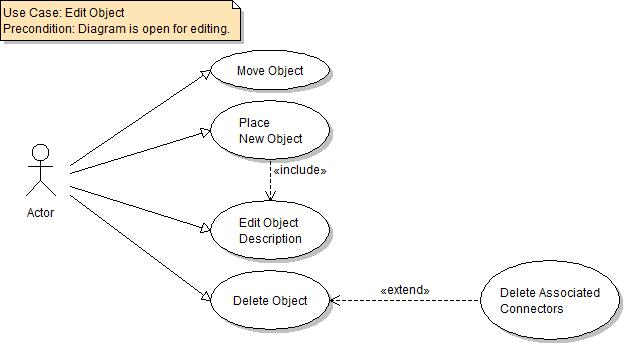
\includegraphics[width=6.0in]{ucaseEditObj.jpg}
\caption{Edit an Object Use Case}
\end{figure}

%%% PLACE NEW OBJECT USE CASE DESCRIPTION
\begin{flushleft}
\tablehead{}
\begin{tabular}{|m{2.0in} m{5.0in}|}
\hline
{\bfseries\emph{Use Case Name}}
& {\bfseries Place New Object}
\\\hline
\emph{Participating Actor}
& User
\\\hline
\emph{Flow of Events}
& \begin{my_enumerate}
\item User selects an object from toolbar.
\item User clicks the canvas.
\item Program places an object at that location on the canvas.
\end{my_enumerate}
\\\hline
\emph{Entry Condition}
& Toolbar is loaded with valid objects for diagram type.
\\\hline
\emph{Exit Condition}
& Object has been successfully placed on drawing canvas.
\\\hline
\emph{Quality Requirements}
& Object may not occupy the same space on the canvas as any other object.
\\\hline
\end{tabular}
\end{flushleft}
\bigskip

%%% EDIT OBJECT DESCRIPTION USE CASE DESCRIPTION
\begin{flushleft}
\tablehead{}
\begin{tabular}{|m{2.0in} m{5.0in}|}
\hline
{\bfseries\emph{Use Case Name}}
& {\bfseries Edit Object Description}
\\\hline
\emph{Participating Actor}
& User
\\\hline
\emph{Flow of Events}
& \begin{my_enumerate}
\item User selects an object by clicking on it.
\item User right-clicks on the object.
\item User selects ``Properties'' from the drop-down menu.
\item User types the desired description in the text box presented.
\item User clicks ``OK.''
\item Program displays new description.
\end{my_enumerate}
\\\hline
\emph{Entry Condition}
& User clicks on an object.
\\\hline
\emph{Exit Condition}
& Program is now showing all user-made changes.
\\\hline
\emph{Quality Requirements}
& There are limitations as to the number of characters a user may enter in the object description text field.
\\\hline
\end{tabular}
\end{flushleft}
\bigskip


%%% MOVE OBJECT USE CASE DESCRIPTION
\begin{flushleft}
\tablehead{}
\begin{tabular}{|m{2.0in} m{5.0in}|}
\hline
{\bfseries\emph{Use Case Name}}
& {\bfseries Move Object}
\\\hline
\emph{Participating Actor}
& User
\\\hline
\emph{Flow of Events}
& \begin{my_enumerate}
\item User clicks on object, selecting it.
\item User holds down the left mouse button, and moves the mouse to the new location of the object.
\item User releases the left mouse button.
\item Program draws the object at the new location, with all attached connectors. 
\end{my_enumerate}
\\\hline
\emph{Entry Condition}
& User selects an object with the left mouse button held down.
\\\hline
\emph{Exit Condition}
& Program has drawn the object at the new location.
\\\hline
\emph{Quality Requirements}
& User may not move an object to a location already occupied by another object. 
\\\hline
\end{tabular}
\end{flushleft}
\bigskip


\clearpage

% ************************************
% EDIT CONNECTOR CASE & DESCRIPTIONS
% ************************************
\paragraph[\ Use Category]
{\ Edit Connector} {These options will be available to the user with a diagram open for modification, who is choosing to take action regarding a connector.}

%%% PLACE NEW CONNECTOR USE CASE DESCRIPTION
\begin{flushleft}
\tablehead{}
\begin{tabular}{|m{2.0in} m{5.0in}|}
\hline {\bfseries\emph{Use Case Name}}
& {\bfseries Place New Connector}
\\\hline
\emph{Participating Actor}
& User
\\\hline
\emph{Flow of Events}
& \begin{my_enumerate}
\item User clicks on desired connector in toolbar.
\item User clicks on the object the connection is coming from, holding down the left mouse button.
\item User drags the mouse toward the object to be connected to.
\item User releases the mouse button.
\item Program draws the connection line between the first and second object.
\end{my_enumerate}
\\\hline
\emph{Entry Condition}
& User has selected a connector from the toolbar.
\\\hline
\emph{Exit Condition}
& The connector is successfully drawn between two objects. 
\\\hline
\emph{Quality Requirements}
& Only one connector may be placed between any two objects. Some objects may not be able to be connected with certain types of connectors.
\\\hline
\end{tabular}
\end{flushleft}
\bigskip


%%% EDIT CONNECTOR PROPERTIES USE CASE DESCRIPTION
\begin{flushleft}
\tablehead{}
\begin{tabular}{|m{2.0in} m{5.0in}|}
\hline {\bfseries\emph{Use Case Name}}
& {\bfseries Edit Connector Properties}
\\\hline
\emph{Participating Actor}
& User
\\\hline
\emph{Flow of Events}
& \begin{my_enumerate}
\item User selects a connector by clicking on it.
\item User right-clicks on the connector.
\item User selects ``Properties'' from the drop-down menu.
\item User edits propertes: 
	\begin{my_enumerate}
\item User types the desired description in the text box presented.
\item User selects desired arrowhead.
\end{my_enumerate}
\item User clicks ``OK.''
\item Program displays new description or arrowhead.
\end{my_enumerate}
\\\hline
\emph{Entry Condition}
& User right clicks on a connector.
\\\hline
\emph{Exit Condition}
& Program has updated the connector with the new properties.
\\\hline
\emph{Quality Requirements}
& Not all connectors will have the same property options.
\\\hline
\end{tabular}
\end{flushleft}
\bigskip


%%% DELETE CONNECTOR USE CASE DESCRIPTION
\begin{flushleft}
\tablehead{}
\begin{tabular}{|m{2.0in} m{5.0in}|}
\hline {\bfseries\emph{Use Case Name}}
& {\bfseries Delete Connector}
\\\hline
\emph{Participating Actor}
& User
\\\hline
\emph{Flow of Events}
& \begin{my_enumerate}
\item User right clicks on a connector.
\item User selects ``Delete'' from the drop-down menu.
\item Program deletes the connector.
\end{my_enumerate}
\\\hline
\emph{Entry Condition}
& User right clicks on the connector.
\\\hline
\emph{Exit Condition}
& Connector has been deleted.
\\\hline
\emph{Quality Requirements}
& TBD
\\\hline
\end{tabular}
\end{flushleft}
\bigskip



\clearpage






\clearpage


\subsubsection[System feature: [Project management tasks suite]{\bfseries System feature: Project management tasks suite}

\paragraph[\ Introduction/Purpose of this feature] {\bfseries Introduction and Purpose of this feature}
{
Several processes are required to manage projects. These include the saving of files, loading projects from files, and deleting projects.}


\paragraph[Input/Output sequence for this feature]{\rmfamily\bfseries Input/Output sequence for this feature}
{
The user selects the ``File'' pull down menu at the top left corner of his or her screen. The options currently supported are ``New'', ``Open'', ``Copy As'', ``Save'', ``Save As'', and ``Delete Project''. }

\subparagraph{New}
{
\\ This creates a new project space. }

\subparagraph{Open}
{
\\ This opens a previously saved project. The user shall be presented with a dialog option to save the previous project. Once completing this dialog, the previous project will be closed and the selected project will be opened.}

\subparagraph{Save}
{
\\ This saves the current state of the project into an XML that can later be used to recreate the project state. If the current project does not have a name, the ``Save'' option will be an alias for the ``Save As'' option.}

\subparagraph{Save As}
{
\\ This creates a new project space and then saves the project state into the new project. In contrast with ``Copy As'', this option does not affect the previous project. }

\subparagraph{Delete Project}
{
\\ This deletes the current project and all files within the project folder. The user shall be presented with a confirmation dialog before this action is completed. Upon completion, a blank and unnamed project will be active in the project window. }









\clearpage\setcounter{page}{1}\pagestyle{Convertvi}
\section[REQUIREMENTS TRACEABILITY]{\rmfamily\bfseries
REQUIREMENTS TRACEABILITY}
{\itshape
}


\bigskip

\begin{flushleft}
\tablehead{\hline
\multicolumn{1}{|m{0.9212598in}|}{\centering
\bfseries Feature Name} &
\centering \bfseries Req No. &
\centering \bfseries Requirement
Description &
\centering \bfseries Priority &
\centering \bfseries SDD &
\multicolumn{2}{m{1.2872598in}|}{\centering
\bfseries Alpha Release} &
\multicolumn{2}{m{1.3587599in}|}{\centering
\bfseries Beta Release} &
\multicolumn{2}{m{1.3795599in}|}{\centering
\bfseries Final Test}\\\hline
 &
 &
 &
 &
 &
\centering \bfseries Test Case(s) &
\centering \bfseries Test Res. &
\centering \bfseries Test Case(s) &
\centering \bfseries Test Res. &
\centering \bfseries Test Case(s) &
\bfseries Test
Res.\\\hhline{~~~~~------}}
\begin{supertabular}{m{0.9212598in}|m{0.42125985in}|m{1.9212599in}|m{0.39275986in}|m{0.7587598in}|m{0.6622598in}|m{0.5462598in}|m{0.6712598in}|m{0.6087598in}|m{0.6712598in}|m{0.6295598in}|}
\multicolumn{1}{|m{0.9212598in}|}{~Select Diagram Type
} &
\centering  1.1 &
~Selects the appropriate diagram type
 &
~M
 &
~N/A
 &
~N/A
 &
~N/A
 &
~N/A
 &
~N/A
 &
~N/A
 &

~N/A
\\\hline
\multicolumn{1}{|m{0.9212598in}|}{~Save function
} &
\centering  2.1 &
~Saves the Diagram to file
 &
~M
 &
~N/A
 &
~N/A
 &
~N/A
 &
~N/A
 &
~N/A
 &
~N/A
 &
~N/A
 
\\\hline
\multicolumn{1}{|m{0.9212598in}|}{~Draw function
} &
\centering  2.1 &
~Draws current objects
 &
~M
 &
~N/A
 &
~N/A
 &
~N/A
 &
~N/A
 &
~N/A
 &
~N/A
 &
~N/A

\\\hline
\multicolumn{1}{|m{0.9212598in}|}{~Open File
} &
\centering  2.1 &
~Opens previously saved file
 &
~M
 &
~N/A
 &
~N/A
 &
~N/A
 &
~N/A
 &
~N/A
 &
~N/A
 &
~N/A

\\\hline
\multicolumn{1}{|m{0.9212598in}|}{~New File
} &
\centering  2.1 &
~Creates New File
 &
~M
 &
~N/A
 &
~N/A
 &
~N/A
 &
~N/A
 &
~N/A
 &
~N/A
 &
~N/A

\\\hline

\multicolumn{1}{|m{0.9212598in}|}{
} &
\centering  2.1 &
~
 &
~
 &
~
 &
~
 &
~
 &
~
 &
~
 &
~
\\\hline

\end{supertabular}
\end{flushleft}
{
Priorities are: \textbf{M}andatory, \textbf{L}ow, \textbf{H}igh}

{
SDD link is version and page number or function name.}

{
Test cases and results are file names and \textbf{P}ass/\textbf{F}ail or
\% passing.}


\end{document}